% !TEX root = sum1.tex
\section{Problem Description}
In this section, to incorporate the social distancing into seat planning, we first give the description of the seat planning problem with social distancing. Then we introduce the dynamic seat assignment problem with social distancing.

% dynamic seat assignment problem, which is suitable for commercial use in cinemas and concerts.

\subsection{Seat Planning Problem with Social Distancing}\label{dynamic_demand}
We consider a layout comprising $N$ rows, with each row containing $S_j$ seats, where $j \in \mathcal{N} \coloneqq \{1,2, \ldots, N\}$. The seating arrangement is intended for various groups, where each group consists of no more than $M$ individuals. There are $M$ distinct group types, denoted by group type $i$ containing $i$ people, where $i \in \mathcal{M} \coloneqq \{1,2, \ldots, M\}$. Represented by a demand vector $\mathbf{d} = [d_1, \ldots, d_M]$, each element $d_i$ represents the number of group type $i$.


In order to comply with the social distancing requirements, individuals from the same group may sit together, while maintaining a distance from other groups. Let $\delta$ denote the social distancing, which could entail leaving one or more empty seats. Specifically, each group must ensure that there are empty seat(s) between them and adjacent groups. Importantly, the seating arrangement of different rows does not affect each other, meaning that individuals from one group can be seated directly behind individuals from another group.

To incorporate the social distancing requirements into the seat planning process, we adjust the original group sizes by adding $\delta$. Consequently, the new size of group type $i$ is denoted as $n_i = i + \delta$, where $i \in \mathcal{M}$. Similarly, to accommodate the adjusted group sizes, the seat layout is modified by adding $\delta$ to the length of each row. Thus, $L_j = S_j + \delta$ represents the length of row $j$, where $S_j$ indicates the number of seats in row $j$. By incorporating the additional seat(s) and designating certain seat(s) for social distancing, we can integrate social distancing measures into the seat planning problem.

The deterministic seat planning problem is formulated below, with the objective of maximizing the number of people accommodated.

\begin{equation}\label{deter_upper}
  \begin{aligned}
  \max \quad & \sum_{i=1}^{M}  \sum_{j= 1}^{N} (n_i- \delta) x_{ij} \\
  \text {s.t.} \quad & \sum_{j= 1}^{N} x_{ij} \leq d_{i}, \quad i \in \mathcal{M}, \\
  & \sum_{i=1}^{M} n_{i} x_{ij} \leq L_j, j \in \mathcal{N} \\
  & x_{ij} \in \mathbb{Z}_{+}, \quad i \in \mathcal{M}, j \in \mathcal{N}.
  \end{aligned}
\end{equation}

This seat planning problem can be viewed as a special case of the multiple knapsack problem. Given the small size of the problem, it is relatively easy to obtain the optimal solution.

To simplify the discussion, we will use a vector $(t_1, \ldots, t_i, \ldots, t_M)$ to represent the pattern, where $t_i$ corresponds to the number of group type $i$. To quantify the effect of each pattern, we introduce the notion of loss, denoting the number of unoccupied seats. 

\begin{prop}\label{lem_pattern}
When given the length of a row, $L$, the social distancing, $\delta$, the adjusted size of the largest group allowed, $n_M$, the loss of the largest pattern is $\lfloor \frac{L}{n_M} \rfloor \delta - \delta + g(L - \lfloor \frac{L}{n_M} \rfloor n_M)$, where $g(r)=0$ if $r> \delta$, and $g(r)= r$ if $r \leq \delta$.
\end{prop}

The loss provides a measure of the number of people who cannot be seated due to the implementation of social distancing constraints. By examining the losses associated with different patterns, we can assess the effectiveness of various seat planning configurations with respect to accommodating the desired number of individuals while adhering to social distancing requirements.

\begin{definition}
Given the length of row and the largest group size, we call the pattern with the minimal loss as the largest patterns. Additionally, we refer to patterns that have no empty seats, except for those reserved for social distancing purposes, as full patterns.
\end{definition}

The largest patterns are characterized by having the least number of people unable to be seated due to social distancing requirements. The full patterns are designed to maximize seating capacity while still maintaining the necessary spacing between groups. 

In most cases, we observe that the optimal solution tends to consist of rows with either full patterns or the largest patterns.
By distinguishing the largest and full patterns from other configurations, we can gain valuable insights into the most efficient seat planning strategies that prioritize accommodating the maximum number of people while adhering to social distancing guidelines.

In scenarios where the demand for seats is high, it is advantageous to adopt the largest pattern, as it allows for the accommodation of a larger number of individuals. The largest pattern becomes particularly beneficial when the demand exceeds the capacity of full patterns. In scenarios where the demand is moderate, adopting the full pattern becomes more feasible. The full pattern maximizes seating capacity by utilizing all available seats, except those required for social distancing measures. Overall, by considering both the largest and full patterns, we can optimize seat planning configurations to efficiently accommodate a significant number of individuals while adhering to social distancing guidelines.

\begin{example}
  Suppose that the social distancing requirement is one seat, and there are four types of groups. In this case, the new sizes of the groups would be 2, 3, 4, and 5, respectively. Additionally, the length of a single row is determined to be L = 21. Then the loss of the largest pattern is $\lfloor \frac{21}{5} \rfloor  - 1 + g(1) = 5$.
  
  We find that the patterns (0, 0, 0, 4), (0, 0, 4, 1), and (0, 2, 0, 3) are the largest patterns with the same loss value of 5. However, it's important to note that the largest pattern may not necessarily be a full pattern. For instance, the pattern (0, 0, 0, 4) is the largest pattern in terms of accommodating the maximum number of individuals, but it does not meet the requirement of fully utilizing all available seats since $4 \times 5 \neq 21$. Conversely, a full pattern may not always be the largest pattern. For example, the pattern (1, 1, 4, 0) is considered a full pattern since it utilizes all seats, but its loss value is 6.
\end{example}


% We consider the social distancing of one empty seat throughout the rest of this paper, which is more practical and reasonable in the seat planning. However, our methods are still applicable to the social distancing of two or more seats.

% Next, we will analyze the impact of implementing social distancing on each row. We define seat planning as the arrangement of seats within a row, specifically, the number of different group types present in each row, as long as the sum of the sizes of all groups is no larger than the length of the row.  

The optimal solution to the seat planning problem can be complex. However, the LP relaxation of problem \eqref{deter_upper} has nice properties.

\begin{prop}\label{sol_relax_deter}
For the LP relaxation of problem \eqref{deter_upper}, there exists $h$ such that the optimal solutions $x_{ij}^{*} = 0$ when $i < h$; $\sum_{j} x_{ij}^{*} = d_{i}$, when $i > h$; $\sum_{j} x_{ij}^{*} = (L - \sum_{i = h+1}^{M} {d_i n_i})/ n_h$, when $i = h$.
\end{prop}

Let $\sum_{j=1}^{N} x_{ij}$ represent the supply for group type $i$. We define $\mathbf{X} = (\sum_{j=1}^{N} x_{1j},\ldots, \sum_{j=1}^{N} x_{Mj})$ as the aggregate solution to the linear relaxation of problem \eqref{deter_upper}. Furthermore, let $e_{i}$ denote the unit size of the $i$-th element of $\mathbf{X}$.

In the aggregate optimal solution, denoted as $x e_{h} + \sum_{i=h+1} ^{M} d_{i} e_{i}$, the following components are present: $x e_{h}$: This term represents the allocation of resources for group type $h$. The value of $x$ is calculated as $(L- \sum_{i = h+1}^{M} {d_i n_i})/ n_h$, indicating the remaining capacity after satisfying the demands of indices greater than $h$, divided by the unit size $n_h$. $\sum_{i=h+1} ^{M} d_{i} e_{i}$: This term accounts for the allocation of resources for group types $h+1$ to $M$. It represents the total demand for these group types, where $d_i$ denotes the demand of group type $i$, and $e_{i}$ represents the unit size of the corresponding element in $\mathbf{X}$. Together, the aggregate optimal solution combines the allocation of resources for group type $h$ with the aggregated demands for group types $h+1$ to $M$ to achieve an optimal solution to the linear relaxation of the problem.


% Therefore, it is crucial to consider both the largest and full patterns separately, as they represent different trade-offs. While the largest pattern maximizes the number of accommodated individuals, the full pattern aims to utilize all available seats. By carefully evaluating these patterns, we can make informed decisions that optimize seat planning configurations while minimizing the loss of seating capacity.

% Then we can illustrate the seat planning for one row below. 
% \begin{figure}[ht]
%     \centering
%     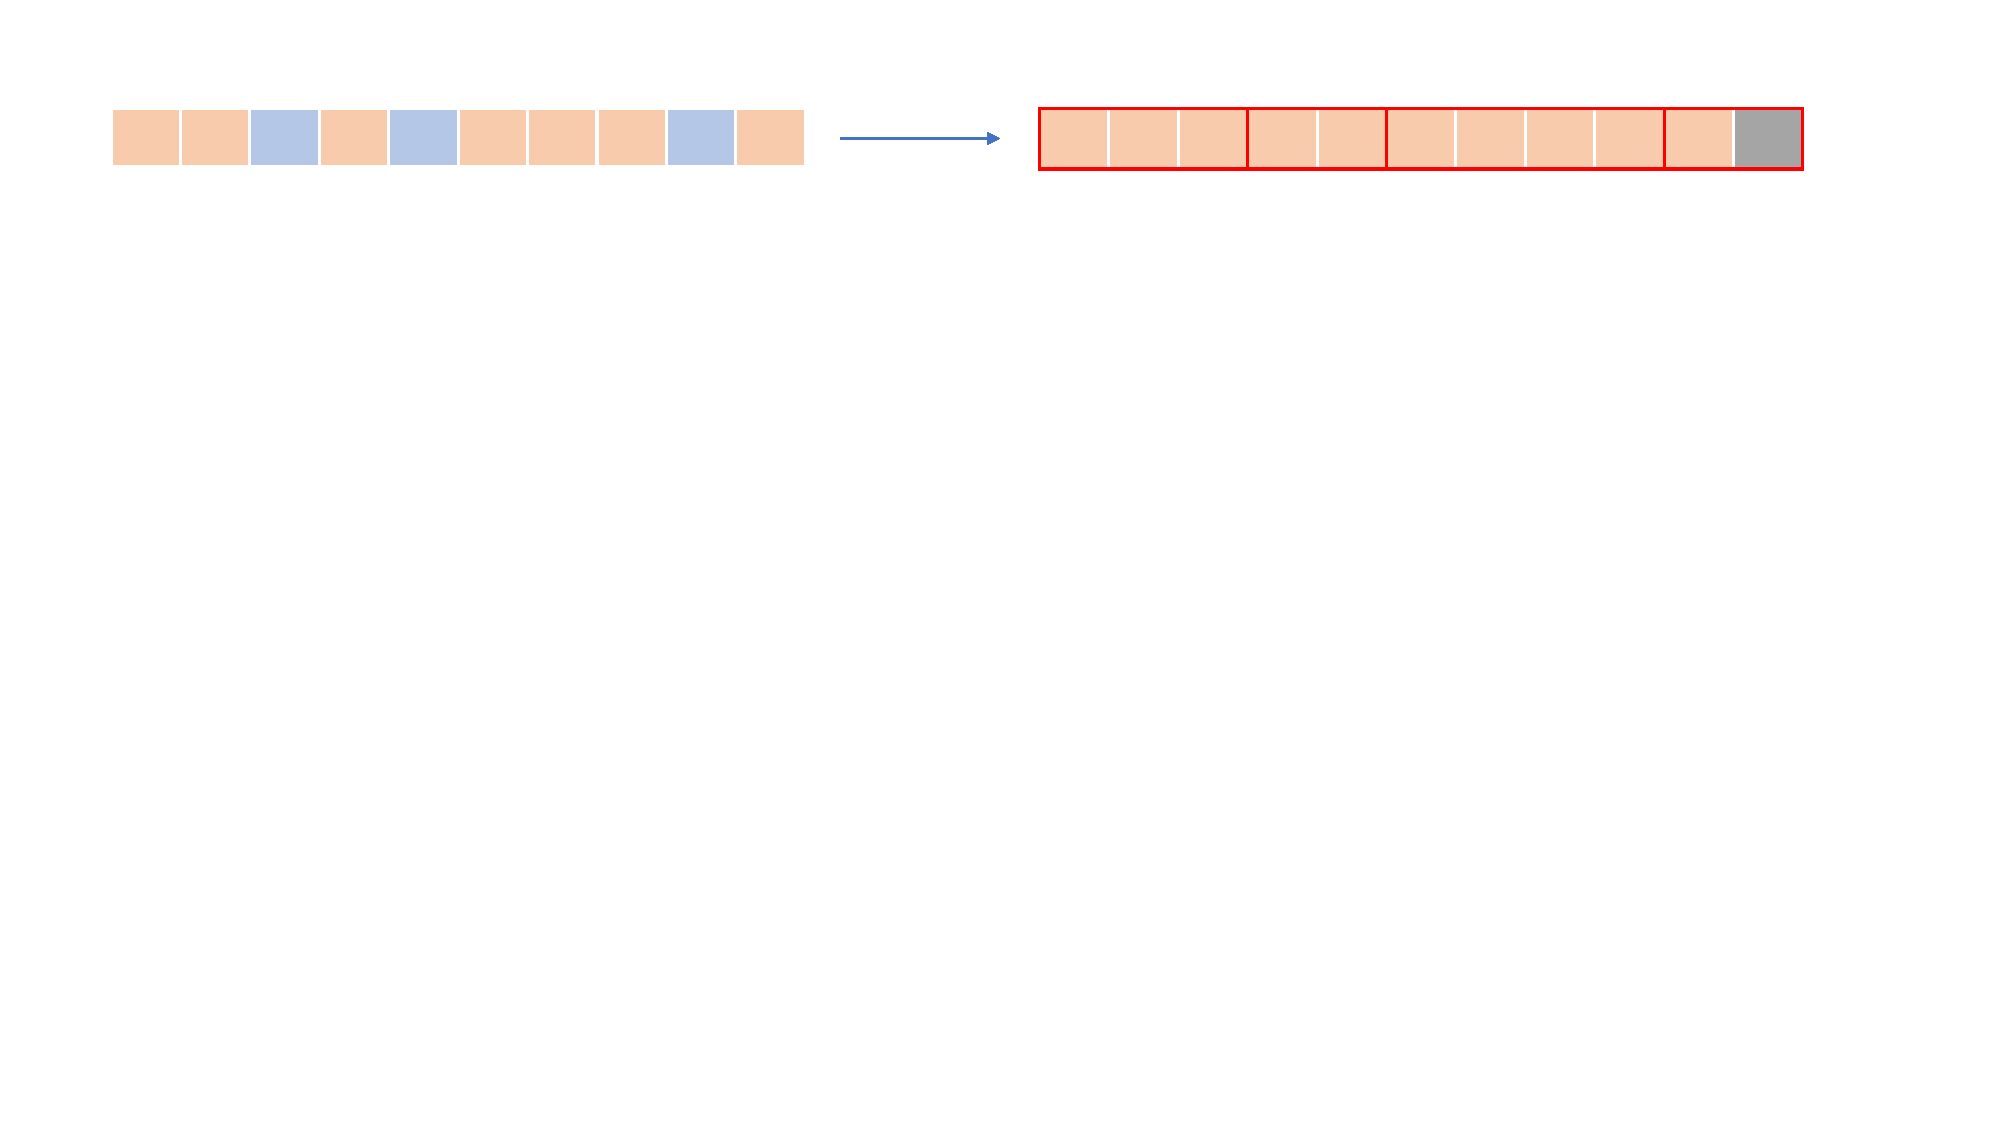
\includegraphics[width = 0.8\textwidth]{./Figures/dummy_seat.pdf}
%     \caption{Problem Conversion}
% \end{figure}

% The social distancing here is one seat. On the left side of the diagram, the blue squares represent the empty seats required for social distancing, while the orange squares represent the seats occupied by groups. On the right side, we have added one dummy seat at the end of each row. The orange squares surrounded by the red line represent the seats taken by groups in this row, which includes two groups of 1, one group of 2, and one group of 3.

% To represent a pattern with a fixed length of form, we can use a $(M+1)-$dimensional vector with $M$ group types. The aggregated form can be expressed as $[n_0, n_1, \ldots, n_M]$, where $n_i$ is the number of $i$-th group type, $i \in \mathcal{M}$. $n_0$ is the number of left seat, its value can only be $0, 1$ because two or more left seats will be assigned to groups. Thus the pattern, $[1, 0, 0, 0, 4]$, is not full because there is one left seat.


% \begin{prop}
% For the seat layout, $\{L_1, L_2, \ldots, L_{N}\}$, the minimal total loss is $\sum_{j} (\lfloor \frac{L_j}{n_{M}} \rfloor \delta -\delta + f(L_j \mod n_{M}))$. The maximal number of people assigned is $\sum_{j} (L_j - \lfloor \frac{L_j}{n_{M}} \rfloor - f(L_j \mod n_{M}))$.
% \end{prop}

\subsection{Dynamic Seat Assignment with Social Distancing}\label{sec_dynamic}
We address the problem of dynamic seat assignment with social distancing, which involves the real-time allocation of seats to incoming groups while ensuring adherence to social distancing guidelines. The decision-maker must make accept or reject decisions for each group and assign them to available seats in rows, while guaranteeing the required spacing between groups. Recalling the seat layout, it consists of $N$ rows, with each row having a length denoted by $L_j$. Additionally, there are $M$ distinct group types, where each group type $i$ consists of $i$ individuals.


To model this problem, we adopt a discrete-time framework. The time is divided into $T$ periods, with each period representing the arrival of exactly one group. Time is discretized as $1, \ldots, T$, where the first period corresponds to the beginning of the selling horizon and the last period represents the end. In each period $t$, a group of size $i$ arrives with a probability denoted as $p_i$. It is assumed that the arrivals of different group types are independent. During each period, the decision-maker determines whether to accept or reject the incoming group and assigns them to a specific row. Once seats are confirmed and assigned to a group, they cannot be changed.

To keep track of the remaining capacity of rows, we utilize a vector $\mathbf{L} = (l_1, l_2, \ldots, l_N)$, where $l_j$ represents the number of remaining seats in row $j$. Specifically, we define $V_t(\mathbf{L})$ as the maximum expected value at period $t$, given the current capacity $\mathbf{L}$. Additionally, we introduce the decision variable $u_{i,j}$, where $u_{i,j}(t) = 1$ denotes the decision to accept group type $i$ in row $j$ at period $t$, while $u_{i,j}(t) = 0$ indicates the rejection of that group type in row $j$ at that period. The decision set is defined as: $U(\mathbf{L}) = \{u_{i,j} \in\{0,1\}, \forall i,j| \sum_{j=1}^{N} u_{i,j} \leq 1, \forall i; n_{i}u_{i,j}\mathbf{e}_j^{\top} \leq \mathbf{L}, \forall i,j \}$. Essentially, $U(\mathbf{L})$ represents the feasible assignment decisions, where each group type $i$ can be assigned to at most one row, and the corresponding capacity requirements are satisfied.

The dynamic programming formula for this problem can be expressed as:

$$V_{t}(\mathbf{L}) = \max_{u_{i,j} \in U(\mathbf{L})}\{ \sum_{i=1}^{M} p_i ( \sum_{j=1}^{N} i u_{i,j} + V_{t+1}(\mathbf{L}- \sum_{j=1}^{N} n_i u_{i,j}\mathbf{e}_j^{\top} ))\}, \mathbf{L} \geq 0, V_{T+1}(\mathbf{L}) =0, \forall \mathbf{L}$$

Here, $\mathbf{e}_j$ represents an N-dimensional unit row vector with $j$-th element being 1. In the above formula, the decision set $U(\mathbf{L})$ represents the feasible set of decisions for a given seat availability $\mathbf{L}$. 

Initially, we have $\mathbf{L} = (L_1, L_2, \ldots, L_{N})$. The objective function is $V_1(\mathbf{L})$. By applying the dynamic programming formula, we can recursively compute the optimal value function $V_t(\mathbf{L})$, representing the maximum expected value at time $t$ for a given seat availability $\mathbf{L}$. This approach allows us to make optimal decisions regarding group acceptance and seat assignment in order to maximize the overall value while considering social distancing constraints and group arrival probabilities. However, this leads to the curse of dimensionality due to the numerous seat planning combinations. To avoid this complexity, we propose an approach that directly targets the final seat planning and then formulate a policy to assign arriving groups. To obtain the final seat planning firstly, we develop the scenario-based stochastic programming.


% Specifically, we define the concept of target seating plans deemed satisfactory. In making the dynamic seating plan, we will try to maintain the possibility of achieving one of the target seating plans as much as possible.
